%
%   SAC参考手册
%   作者:SeisMan
%   网址:http://seisman.info/sac-manual.html
%   编译环境:TeXLive 2013
%   中文支持:xeCJK + xeLaTeX
%

\documentclass[a4paper, 11pt, twoside]{book}
%
% LaTeX配置文件
% 

% 文档相关信息
\newcommand{\SACDOCTITLE}{SAC\textbf{参考手册}} % 文档标题
\newcommand{\SACDOCAUTHOR}{SeisMan}             % 文档作者
\newcommand{\SACDOCVERSION}{3.0}                % 文档版本
\newcommand{\SACDOCDATE}{\today}                % 文档更新日期

% SAC相关信息
\newcommand{\SACVERSION}{101.6a}                % 文档对应的SAC版本
\newcommand{\SACDATE}{2013-11-11}               % SAC的发布日期

% 中文支持及中英文字体设置
\usepackage[
    indentfirst,    % 章节标题后首段缩进
    CheckSingle,    % 避免单个CJK字符位于段落最后一行
]{xeCJK}
\setmainfont[Mapping=tex-text]{Adobe Garamond Pro}
\setCJKmainfont[BoldFont={Adobe Heiti Std},
    ItalicFont={Adobe Kaiti Std}]{Adobe Song Std}
\setCJKsansfont{Adobe Heiti Std}
\setCJKmonofont{Adobe Fangsong Std}

% 页面设置
\usepackage[top=3.0cm,bottom=2.0cm,left=3.5cm,right=2.5cm]{geometry}

% 间距设置
\linespread{1.3}                        % 行间距
\addtolength{\parskip}{3pt}             % 段落间距
\addtolength{\abovecaptionskip}{-3pt}   % caption上间距
\addtolength{\belowcaptionskip}{-3pt}   % caption下间距
\setlength{\parindent}{2em}             % 首行缩进

% 标题设置
\usepackage{titlesec}
% 设置章格式
\titleformat{\chapter}{\centering\Huge\bfseries}{第\,\thechapter\,章}{1em}{}
% 调整subsection前后间距
\titlespacing*{\subsection}{0ex}{-.2ex}{.2ex}
%设置SACTitle为subsection格式
\newcommand{\SACTitle}[1]{\subsection*{#1}}		

% 目录设置
\usepackage{titletoc}
\setcounter{tocdepth}{1}
\titlecontents{chapter}[0em]
{\vspace{0.2em}\bfseries\Large}
{第\,\thecontentslabel\,章\quad}
{\hspace*{0em}}
{\hfill \contentspage}
\titlecontents{section}[1em]
{\large}
{\thecontentslabel\quad}
{\hspace*{0em}}
{\ \dotfill \ \contentspage}
[\vspace{-0.3em}]

% 页眉页脚设置
\usepackage{titleps}
\newpagestyle{main}{
    \sethead
    [$\cdot$~\thepage~$\cdot$][][\small\S\,\thesection\quad\sectiontitle]
    {第\,\thechapter\,章\quad\chaptertitle}{}{$\cdot$~\thepage~$\cdot$}
    \setfoot{}{}{}\headrule
}

% 空白页	
\makeatletter	% copy from lnotes
\def\cleardoublepage{
    \clearpage
    \if@twoside
        \ifodd
            \c@page
        \else
            \hbox{}
            \vspace*{\fill}
            \begin{center}
		    我是空白页,双面打印更环保
            \end{center}
            \vspace{\fill}
            \thispagestyle{empty}
            \newpage
            \if@twocolumn
                \hbox{}
                \newpage
            \fi
        \fi
    \fi
}
\makeatother

% 脚注
\usepackage[perpage]{footmisc}	% 脚注在每一页单独编号

% 超链接及书签
\usepackage[bookmarks=true,colorlinks,linkcolor=blue, citecolor=blue]{hyperref}
\hypersetup{ % 文档元信息
    pdftitle={\SACDOCTITLE v\SACDOCVERSION},
    pdfauthor={\SACDOCAUTHOR},
}

% 表格
\usepackage{booktabs}
\usepackage{multirow}
\usepackage{longtable}
\renewcommand\arraystretch{1.0}	    % 表格行间距

% 代码宏包
\usepackage{listings}	
\usepackage[usenames,dvipsnames,svgnames]{xcolor} % 用于code
\lstloadlanguages{[77]Fortran,[ANSI]C,Perl,Python,bash,csh} % 载入所有需要的语言
% lstings的默认设置, 主要用于lstinline
\lstset{
    basicstyle=\ttfamily,	% 使字体保持当前的系列与形状属性,但转变为打字机族属性
}
\setmonofont{Droid Sans Mono}
% 单行代码
\lstdefinestyle{Shell} {
    basicstyle=\scriptsize\ttfamily,
    xleftmargin=4em,
    xrightmargin=4em,
    showspaces=false,
    breakatwhitespace=false,
    breaklines=true,
    commentstyle=\color[rgb]{0,0.6,0},
    keywordstyle=\color{blue},
    frame=leftline,
%    frame=single,
    framerule=1pt,
    numbers=none,
    rulecolor=\color{blue},
    showspaces=false,
    showstringspaces=false,
    showtabs=false,
    stepnumber=1,
    stringstyle=\color[rgb]{0.58,0,0.82},
    tabsize=4
}
% 函数声明
\lstdefinestyle{FunctionDeclaration} {
    basicstyle=\small\ttfamily,
    xleftmargin=2em,
    xrightmargin=2em,
    showspaces=false,
    breakatwhitespace=false,
    breaklines=true,
    commentstyle=\color[rgb]{0,0.6,0},
    keywordstyle=\color{blue},
    frame=shadowbox,
    numbers=none,
    rulecolor=\color{black},
    rulesepcolor=\color{blue},
    showspaces=false,
    showstringspaces=false,
    showtabs=false,
    stepnumber=1,
    stringstyle=\color[rgb]{0.58,0,0.82},
    tabsize=4
}
% 函数定义
\lstdefinestyle{FunctionDefinition} {
    basicstyle=\small\ttfamily,
    xleftmargin=2em,
    xrightmargin=2em,
    showspaces=false,
    breakatwhitespace=false,
    breaklines=true,
    commentstyle=\color[rgb]{0,0.6,0},
    keywordstyle=\color{blue},
    frame=shadowbox,
    numbers=left,
    numbersep=5pt,
    numberstyle=\small\color[rgb]{0.5,0.5,0.5},
    rulecolor=\color{black},
    rulesepcolor=\color{blue},
    showspaces=false,
    showstringspaces=false,
    showtabs=false,
    stepnumber=1,
    stringstyle=\color[rgb]{0.58,0,0.82},
    tabsize=4
}
\lstdefinelanguage{SAC} {
%    keywords={SAC},
    otherkeywords={SAC>},   % SAC提示符
    sensitive=true,
    comment=[l][{\color[rgb]{0,0.4,0}}]{//},
    morecomment=[s]{/*}{*/}
}
\lstnewenvironment{SACCode}{
    \lstset{
        language={SAC},                     % 语言
        basicstyle=\small\ttfamily,         % 字体
        xleftmargin=2pc,                    % 整体布局
        xrightmargin=2pc,
        %lineskip=0pt,                      % 行间距
        backgroundcolor=\color{Lavender},   % 背景色
        frame=single,                       % 边框
        rulecolor=\color{Silver},           % 边框颜色
        keywordstyle=\color{blue},          % 关键字颜色
    }
}{}

% 列表
\usepackage{enumitem}	% 列表宏包
% itemsep 设置列表间距
% topsep 设置列表前间距
\setenumerate[1]{itemsep=0pt,partopsep=0pt,parsep=\parskip,topsep=0pt}
\setitemize[1]{itemsep=-2pt,partopsep=0pt,parsep=\parskip,topsep=0pt}
\setdescription{itemsep=-5pt,partopsep=0pt,parsep=\parskip,topsep=0pt,itemindent=0pt}

% 定义\today的格式
\usepackage[yyyymmdd]{datetime}
\renewcommand{\dateseparator}{-}

% 抄录
\usepackage{verbatim}

% 图片
\usepackage{graphicx}
\graphicspath{{figures/}}

% 汉化
\renewcommand{\contentsname}{目 \quad 录}
\renewcommand{\listfigurename}{图目录}
\renewcommand{\listtablename}{表目录}
\renewcommand{\figurename}{图}
\renewcommand{\tablename}{表}
\renewcommand{\bibname}{参考文献}
\renewcommand{\indexname}{索引}
\renewcommand{\figureautorefname}{图}
\renewcommand{\tableautorefname}{表}
\renewcommand{\appendixautorefname}{附录}


\begin{document}

\begin{titlepage}
\begin{center}
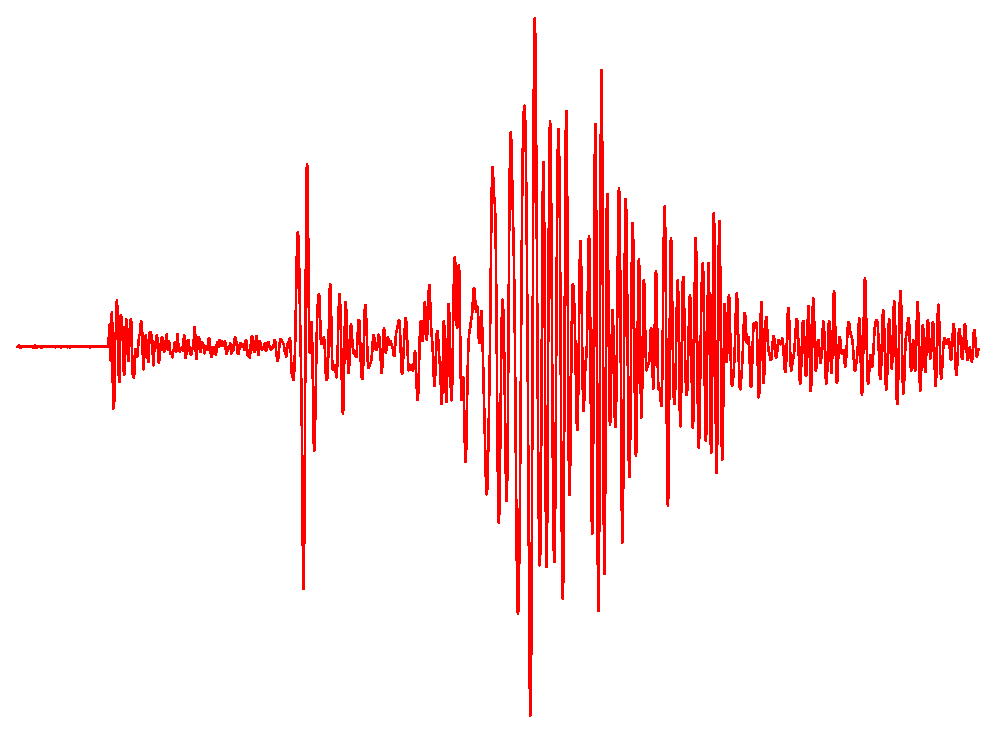
\includegraphics[width=0.8\textwidth]{SAC_logo}\\
\rule{8cm}{0.5mm}\\[0.35cm]
\Huge{\SACDOCTITLE}\\
\rule{8cm}{0.5mm}\\
\Large{\hspace{2.5cm} 基于SAC v\SACVERSION}\\[1cm]

\begin{minipage}{0.8\textwidth}
\begin{flushright}
\begin{tabular}{cl}
\emph{作者:} & \SACDOCAUTHOR \\
\emph{版本:} & \SACDOCVERSION \\
\emph{日期:} & \SACDOCDATE	\\
\end{tabular}
\end{flushright}
\end{minipage}
\end{center}

\end{titlepage}

\pagestyle{empty}

\frontmatter
\section*{\centering 写在第三版前的一些废话}

\begin{shadequote*}
\Large\emph{
工欲善其事,必先利其器。
}
\par\hfill\emph{\normalsize---《论语 $\cdot$ 卫灵公》}
\end{shadequote*}

2010年10月,大三,开始接触并学习SAC;2011年的暑假
开始着手SAC文档的翻译工作;2012年01月,文档的v1.0版本发布;2013年03月
,文档的v2.0版发布。3年多的时间过去了,文档更新到了v3.0版。

v2.0大体上算是官方英文文档的译本,整体结构上完全遵循了官方文档的风格。
整个文档的条理不够清晰,教程部分稍显单薄,命令部分也不够完善。

2013年11月,George Helffrich著的
``\emph{The Seismic Analysic Code : A Primer and User's Guide}''一书出版了。
该书基于MacSAC,与本文档所关注的SAC有一些区别,但是精髓部分是一致的。
v3.0版借鉴了该书的整体结构和部分内容,重新设计了文档结构并重写了教程的大
部分内容,希望能够有一个结构更清晰、内容更丰富的版本。

整个文档分为教程部分和命令部分。教程部分又分为如下几章:
\begin{description}
\item[SAC简介] 简单介绍SAC软件的相关信息;
\item[SAC基础] 继续阅读所需的基础知识;
\item[SAC文件格式] 详细介绍SAC文件格式;
\item[SAC数据处理] 介绍如何利用SAC命令进行地震数据处理和分析;
\item[SAC图像] 介绍如何控制SAC绘制的图像的细节;
\item[SAC编程] 介绍如何用SAC进行数据批处理;
\item[SAC与脚本] 如何在脚本语言(Bash和Perl)中调用SAC;
\item[SAC函数库] 在自己的C或Fortran程序中调用SAC提供的子函数;
\item[SAC I/O] 独立实现SAC I/O子函数;
\item[SAC相关工具] 与SAC有关的一些工具;
\end{description}

对本文档的内容有疑问,或发现任何错误、笔误,欢迎邮件联系我或者在本文档的
GitHub项目主页上提交Issue,也欢迎感兴趣的读者fork该项目,共同完善文档。

此文档仅供个人学习使用,希望不涉及版权问题。

\begin{flushleft}
个人博客: \url{http://seisman.info}                                     \\
项目主页: \url{https://github.com/seisman/SAC_Docs_zh}                  \\
捐赠页面:\url{https://me.alipay.com/seisman}                           \\
文档发布页: \url{http://seisman.info/sac-manual.html}                   \\
联系方式: \url{seisman.info@gmail.com}  

\end{flushleft}

\begin{flushright}
作者~:~SeisMan \\
2014年04月14日
\end{flushright}

\section*{\centering{版本}}

SAC的开发一直在进行,每一个新版本都可能修订一些Bug、加入一些新的特性或
增加新的命令。下表列出了本文档的版本与SAC版本之间的对应关系。就本文档而言,
推荐读者使用SAC的v101.5c或v101.6a版本。

\begin{table}[h]
\centering
\begin{tabular}{c|c|c|c}
\toprule
文档版本		& 	文档发布日期 	& 	SAC版本 &	SAC 发布日期\\
\midrule
1.0  			&	2012-01-08		&	101.4	&	2010-06-07	\\
1.1  			&	2012-09-03		&	101.4	&	2010-06-07	\\
1.2  			&	2012-09-18		&	101.5	&	2011-11-15	\\
2.0  			&	2013-03-29		&	101.5c	&	2012-02-01	\\
2.1  			&	2013-04-06		&	101.5c	&	2012-02-01	\\
2.2  			&	2013-04-12		&	101.5c	&	2012-02-01	\\
2.3             &   2014-02-22      &   101.5c  &   2012-02-01  \\
\SACDOCVERSION  &   \SACDOCDATE     &   \SACVERSION &   \SACDATE    \\
\bottomrule
\end{tabular}
\end{table}


\frontmatter
\tableofcontents
\listoffigures
\listoftables

\mainmatter
\pagestyle{body}

\chapter{SAC简介}
\section{SAC是什么?}

Seismic Analysis Code (SAC),是地震学领域使用最广泛的数据分析软件包之一。

SAC首先是一个软件,主要在命令行下工作,通过各种命令来处理时间序列数据
(尤其是地震数据),同时也包含了一个简单的图形界面,使得用户可以方便地查看
波形以及拾取震相。

SAC同时还是一种数据格式,定义了以何种方式存储单个时间序列数据。
SAC格式已经成为了地震学的标准数据格式之一,有很多工具可以实现SAC格式
与其它地震数据格式间的相互转换。

SAC实现了地震数据处理过程中的常用操作,包括重采样、插值、自/互相关、震相拾取、
快速Fourier变换、谱估计、滤波、信号叠加等;同时为了满足数据批处理的需求,
SAC设计了一个基本的编程语言,包括变量、参数、If判断、循环等等
\footnote{SAC设计的基本编程语言,称之为SAC宏,在第\ref{chap:macros}章中会详细
说明,并与Bash和Perl进行对比。}。

\section{SAC发展史}
\label{sec:history}

Lawrence Livermore国家实验室
\footnote{\url{http://en.wikipedia.org/wiki/Lawrence\_Livermore\_National\_Laboratory}}
和Los Alamos国家实验室
\footnote{\url{http://en.wikipedia.org/wiki/Los\_Alamos\_National\_Laboratory}}
是美国承担核武器设计工作的两个实验室。SAC于20世纪80年代诞生于实验室的Treaty Verification Program小组里,该组由W. C. Tapley和Joe Tull共同领导。

起初,SAC是用Fortran语言实现的,并将源代码分发给感兴趣的学者,
允许用户进行非商业性的地震数据处理,
用户和开发者之间的合作协议要求用户提交bug修正和改进以换取SAC的使用权。
到了大概1990年,SAC已经成为全球地震学家的数据处理标准软件。

从1992年开始,SAC的开发逐渐由Livermore接管,并开始通过分发协议严格限制源代码的
分发。与此同时,开发者认为Fortran是一种过于局限的编程语言,其阻碍了SAC特性的进一步
开发,因而开发者使用f2c\footnote{f2c~(\url{http://www.netlib.org/f2c/}),
Fortran77语言到C语言的自动转换工具。}
转换工具将SAC的Fortran源码转换成了C源码\footnote{个人猜测,目前SAC源码的
混乱和不易读正是由于这次自动转换导致的。}。接下来,Livermore以转换得到的
C源码为基础,计划开发一个商业版的地震数据处理产品,命名为SAC2000。
这个版本扩展了很多
功能,其中一个功能是建立一个日志数据库,记录一个波形从原始数据
到最终产品之间的所有处理步骤。这样的设计允许用户暂时保存数据处理步骤,
随时将处理的结果提交到内存或回滚到之前的状态。

约1998年,IRIS\footnote{\url{http://www.iris.edu}}
意识到,SAC的核心用户群(主要是IRIS的成员)无法确保能够
获取SAC的源码。IRIS开始和Livermore协商,希望将SAC的开发分成两条线:一个包含
数据库特性,供核监测机构使用;另一个不包含数据库特性,仅供学术机构使用。
商业化的努力主要集中在含数据库功能的版本上。

终于,在2005年,IRIS与Livermore签订了合同,Livermore提供给IRIS一个SAC协议,
允许其在IRIS社区
内部分享SAC/SAC2000的源代码,并提供有限的支持以促进社区的发展。
而学术圈对于商业版的SAC没有太大兴趣,因而Livermore逐渐撤出了对于SAC2000的支持。
最终IRIS完全接手了SAC的开发和技术支持,并成为了一个新的版本,
也就是我们现在正在使用的SAC,有时为了区分,也称之为SAC/IRIS。
目前的最新版本为101.6a。

\section{SAC变体}

SAC的发展史还是很曲折的,这也导致SAC存在多个不同的变体。

\begin{description}
\item[Fortran SAC]  即SAC的Fortran语言实现。最后一个分发版本发布于2003年,版本号10.6f。
                    曾经以限制性的形式在IASPEI软件库中分发。
\item[SAC2000]      从Fortran源码转换为C源码,并以C源码为基础继续维护。该版本加入了数据库特性以及
                    一些新的命令。目前该版本已不再分发。
\item[SAC/IRIS]     由SAC2000衍生的版本,不包含数据库特性\footnote{目前的SAC/IRIS中还可以看到一些
                    与数据库特性相关的命令和选项,比如很多命令中的commit、rollback、recalltrace选项,
                    这些选项的存在属于历史遗留问题,且已经基本不再维护,因而本文档中完全没有提及。},
                    也就是本文档所使用的版本,在本文档中简称为SAC。
                    现在由IRIS下的SAC开发小组负责维护,并由IRIS分发。
\item[MacSAC]       也称为SAC/BRIS,仅可在Mac OS下使用。该变种由10.6d Fortran源码衍生而来(后期与10.6f集成),
                    其功能是SAC/IRIS功能的超集。相对于SAC/IRIS的最主要扩展在于宏语言功能的增强以及
                    处理台阵数据的能力。其作者为
                    George Helffrich\footnote{\url{http://www1.gly.bris.ac.uk/~george/gh.html}},
                    针对MacSAC写了一本教程
                    \footnote{G.R. Helffrich, J. Wookey \& I.D. Bastow, The Seismic Analysis Code
                    : A Primer and User's Guide. \textsl{Cambridge University Press}, 2013。
                    可以作为学习SAC/IRIS的辅助教程,但需要注意其中可能存在的一些微小差异。}。
\end{description}

\section{安装SAC}
\label{sec:sac-install}
本节介绍如何在Linux下安装SAC,要求读者了解Linux的一些基本概念和操作。

\subsection*{申请SAC}
在``\nameref{sec:history}''中已经说到,SAC协议仅允许在IRIS社区内部分享SAC的源码,
所以SAC不像很多软件一样可以很方便地通过软件包管理器安装或者直接从网络下载源码。

软件包申请地址~:~\url{http://www.iris.edu/ds/nodes/dmc/forms/sac/}

认真填写个人信息,尤其注意Email那一栏,需要填写单位邮箱,如果使用
QQ、163这样的邮箱很容易直接被拒绝,如果没有单位邮箱,需要提供其它
信息以验证你的身份。

IRIS提供了SAC源码包、Linux 64位二进制包和Mac 64位二进制包。对于Linux
用户,可以通过``\lstinline{uname -a}''命令查看当前系统是32位还是64位。对于64位系统,
可以直接使用Linux 64位二进制包;对于Linux 32位系统,则必须手动编译SAC源码。

考虑到在申请提交之后,需要人工审核,两三个工作日后才会通过邮箱获取SAC软件包,
建议还是同时申请Linux 64位二进制包和SAC源码包。

\subsection*{安装依赖包}
Linux下安装软件最麻烦的一个问题就是软件之间的依赖关系。

对于Ubuntu/Debian系\footnote{很久不用Ubuntu,无法保证完全正确。}:
\begin{lstlisting}[style=Shell]
$ sudo apt-get install build-essential
$ sudo apt-get install libncurses5-dev libsm-dev libice-dev
$ sudo apt-get install libxpm-dev libx11-dev zlib1g-dev
\end{lstlisting}

对于CentOS/Fedora/RHEL系:
\begin{lstlisting}[style=Shell]
$ sudo yum groupinstall 'Development Tools'
$ sudo yum install glibc ncurses-devel libSM-devel libICE-devel
$ sudo yum install libXpm-devel libX11-devel zlib-devel
\end{lstlisting}

\subsection*{安装}
安装的方法在这一步分成两个部分,分别是二进制包安装和源代码编译,根据实际情况
二者选一。
\subsubsection*{二进制包安装}
解压sac二进制包:
\begin{lstlisting}[style=Shell]
$ tar -zxvf sac-101.6a-linux_x86_64.tar.gz
\end{lstlisting}

复制sac文件夹到安装目录(推荐安装目录为\lstinline{/usr/local}):
\begin{lstlisting}[style=Shell]
$ sudo cp -r sac /usr/local
\end{lstlisting}

\subsubsection*{源代码编译}
\begin{lstlisting}[style=Shell]
$ tar -zxvf sac-101.6a_source.tar.gz
$ cd sac-101.6a
$ ./configure --prefix=/usr/local/sac
$ make
$ sudo make install
\end{lstlisting}

\subsection*{配置变量}
向~\lstinline{~/.bashrc}~中加入如下语句以配置环境变量和SAC全局变量:
\begin{lstlisting}[style=Bash]
export SACHOME=/usr/local/sac
export SACAUX=$SACHOME/aux
export PATH=$SACHOME/bin:$PATH

export SAC_DISPLAY_COPYRIGHT=1
export SAC_PPK_LARGE_CROSSHAIRS=1
export SAC_USE_DATABASE=0
\end{lstlisting}

其中,
\begin{itemize}
\item \lstinline{SACHOME}~为SAC的安装目录;
\item \lstinline{SACAUX}~中包含了SAC运行所需的辅助文件;
\item \lstinline{PATH}~为Linux系统环境变量;
\item \lstinline{SAC_DISPLAY_COPYRIGHT}~用于控制是否在启动SAC时显示版本和版权信息,
    一般设置为1。在脚本中多次调用SAC时会重复显示版本和版权信息,干扰脚本的正常输出,因而
    在脚本中一般将其值设置为0,设置方法可以参考``\nameref{sec:sac-bash}''、``\nameref{sec:sac-perl}''和``\nameref{sec:sac-python}''
    中的相关内容;
\item \lstinline{SAC_PPK_LARGE_CROSSHAIRS}~用于控制震相拾取过程中光标的大小,在
    ``\nameref{sec:phase-picking}''一节会具体说明;
\item \lstinline{SAC_USE_DATABASE}~用于控制是否允许将SAC格式转换为GSE 2.0格式;
    一般用不到该特性,故而设置其值为0;
\end{itemize}

修改完~\lstinline{~/.bashrc}~后,执行以下命令使配置的环境变量生效:
\begin{lstlisting}[style=Shell]
$ source ~/.bashrc
\end{lstlisting}

\subsection*{启动SAC}
终端键入小写的sac\footnote{Ubuntu的源里有一个名叫sac的软件,是用来显示登录账户
的一些信息;CentOS的源里也有一个名叫sac的软件,是CSS语法分析器的Java接口。所以
一定不要试图用发行版自带的软件包管理器安装sac!!!},显示如下则表示SAC安装成功:
\begin{lstlisting}[style=Shell]
$ sac
 SEISMIC ANALYSIS CODE [11/11/2013 (Version 101.6a)]
 Copyright 1995 Regents of the University of California

SAC>
\end{lstlisting}

\section{邮件组}
邮件组是个好东西,有点我们熟悉的QQ群的味道。在加入了邮件组之后,如果你在使用SAC的过程中
遇到问题,
可以向这个邮件组的邮箱发送HELP邮件,该组内的所有成员都会收到你的邮件。
如果某人知道答案,他或许就会给你回复。发现了SAC的bug也可以向这里报告,开发者会尽快给你回复的。
当然问问题之前要思考
\footnote{请阅读<提问的智慧>\url{http://www.wapm.cn/smart-questions/smart-questions-zh.html}},
提交bug的时候要详细指出bug是如何出现的,也可以给出代码或文件以使得开发者能够重现该bug。

邮件组邮箱~:~\url{sac-help@iris.washington.edu}

订阅地址~:~\small{\url{http://www.iris.washington.edu/mailman/listinfo/sac-help}}


\chapter{SAC基础}
\section{如何学习SAC?}
学习SAC最好的方式是找一个有经验且有耐心的人,让他/她给你演示SAC是如何工作的。
如果没有这样一个人的话,那么你就需要打开终端从头开始自学。

我将SAC的学习过程分成三个阶段,下面列出了每个阶段的具体要求。普通用户需要达到``SAC进阶''
才能满足日常数据处理的要求。

\subsection*{SAC初阶}
\begin{enumerate}
    \item 掌握SAC中最常用的命令,包括但不限于
            \nameref{cmd:help}、
            \nameref{cmd:read}、
            \nameref{cmd:write}、
            \nameref{cmd:plot}、
            \nameref{cmd:quit}、
            \nameref{cmd:plotpk}、
            \nameref{cmd:listhdr}、
            \nameref{cmd:chnhdr}、
            \nameref{cmd:rmean}、
            \nameref{cmd:rtrend}、
            \nameref{cmd:bandpass}、
            \nameref{cmd:plot1}、
            \nameref{cmd:plot2}、
            \nameref{cmd:cut}、
            \nameref{cmd:fft};
        \item 理解地震数据处理流程,参见``~\nameref{chap:data-process}''一章;
        \item 了解~\nameref{chap:sac-file-format},掌握常见的~\nameref{sec:sac-header-variables},
            理解~\nameref{sec:sac-time};
        \item SAC相关工具:\nameref{sec:saclst};
\end{enumerate}

\subsection*{SAC进阶}
\begin{enumerate}
\item 掌握SAC的大部分命令,至少知道SAC可以实现哪些功能;
\item 了解SAC编程以及如何在脚本中调用SAC,见第~\ref{chap:sac-programming}~、~\ref{chap:sac-script}~章;
\item 掌握如何绘制精美的波形图,见第~\ref{chap:sac-graphics}~章;
\item 学会在自己的程序中使用SAC提供的函数库,见第~\ref{chap:sac-libs}~章;
\end{enumerate}

\subsection*{SAC高阶}
\begin{enumerate}
\item 了解SAC软件包的内部结构;
\item 自己写程序实现SAC I/O库;
\item 阅读SAC源码,了解命令的技术细节;
\item 向SAC贡献代码;
\end{enumerate}

\section{如何阅读本文档?}

本文档的内容大体分为两个部分:教程部分和命令部分。命令部分详细的列出了SAC中的
每一个命令的语法、参数以及一些技术细节,适合作为参考,在需要的时候查阅。

教程部分给出了很多日常数据处理的例子,初学者应该坐在计算机前,打开终端,
键入\footnote{严禁复制!不许偷懒!}书中的例子,试着理解每一个步骤的原理以及结果。

在阅读教程的同时,应随时翻看相应命令的说明,在实践的过程中掌握基础命令的语法和用法。
这样基本就完成了SAC初阶的要求。

在读完教程部分之后,应浏览SAC的几乎所有命令,并挑选其中感兴趣的一些进行尝试。此后,
在平常的科研工作中经常使用SAC,有了实践经验和对SAC的进一步认识之后,可以阅读文档
中的进阶内容,达到SAC进阶的要求。

最后,如果对SAC的内部机理感兴趣,可以阅读SAC的源码,重新实现一些SAC底层的功能。

\section{启动和退出}
在终端键入\lstinline{sac}以启动SAC,显示如下版本号以及版权信息
\footnote{Livermore实验室由University of California于1952年创立,2007年改由
University of California、Bechtel National、BWX Technologies、Washington Group International
共同组成的安全机构管理。}
:
\begin{SACCode}
$ sac
 SEISMIC ANALYSIS CODE [11/11/2013 (Version 101.6a)]
 Copyright 1995 Regents of the University of California

SAC> 
\end{SACCode}
其中, ``\lstinline{SAC>}''是SAC程序特有的提示符。

退出SAC:
\begin{SACCode}
SAC> quit
\end{SACCode}
也可以使用\lstinline{done}、\lstinline{exit}命令退出SAC,但不推荐。

\section{SAC设计思想}
SAC的设计思想大概可以总结如下:
\begin{enumerate}
    \item 每个信号\footnote{信号,或称之为trace,即\textbf{单个}台站\textbf{单个}仪器\textbf{单个}分量的数字记录。}
被保存到单独的SAC格式数据文件中;
\item SAC格式包含了描述数据特征的头段区和存储信号的数据区,参见``~\nameref{chap:sac-file-format}~''一章;
\item 将单个或多个\footnote{一次性最多处理\textbf{1000}个任意大小的文件,记住1000这个值!}
    SAC文件从磁盘读入内存;
\item 通过各种命令对内存中的数据进行操作;
\item 操作完毕,将内存中的数据写入到磁盘,可以覆盖原SAC文件或写入新文件中。
\end{enumerate}

\section{SAC命令初探}
\subsection{SAC命令长什么样?}
一个完整的SAC命令一般由``命令+选项+参数''构成,其中命令必须有,选项和参数可以成对
出现,也可以只出现其中一个。命令、选项以及参数之间用空格分开。如果要将多个命令写在
一行,要用分号隔开每个命令。例如:
\begin{SACCode}
SAC> funcgen random delta 0.1 npts 1000
SAC> rmean; rtrend; taper                 // 一行内多个命令用分号隔开
SAC> write rand.SAC
\end{SACCode}
其中,~\lstinline{funcgen}~、~\lstinline{write}~、~\lstinline{rmean}~、~\lstinline{rtrend}~
和~\lstinline{taper}~是命令;~\lstinline{random}~是选项;
~\lstinline{0.1}~是选项~\lstinline{delta}~的参数、~\lstinline{1000}~是选项
~\lstinline{npts}~的参数;而~\lstinline{rand.SAC}~则是一个无选项的参数\footnote{其实
可以有很多选项,这里都省略了。}。

\begin{Tips}
官方文档的原文是``command''、``keyword''和``option'',
本文档v2.0中译为``命令'',``关键字''和``参数''。
个人感觉,无论是官方的用词还是v2.0版的译词都很容易让使用C语言和Linux的人困惑,
因而v3.0中一律将其改为命令(command)、选项(option)和参数(argument)。

这里解释一下选项(option)和参数(argument)的区别。一个命令有哪些选项是由命令规定的,
其控制了命令的一些特性,因而选项的作用是告诉命令``我\textbf{要}改某个特性''。
但是具体\textbf{怎么}改呢?
这个就交给参数来控制了。命令或选项只规定了参数的类型(整型、浮点型、字符串、枚举型或者逻辑型),
用户需要根据自己的需求给定参数值。
\end{Tips}

\subsection{大小写}
SAC的命令和选项都是不区分大小写的,这意味着你可以根据自己的喜好使用~\lstinline{funcgen}~
或者~\lstinline{FUNCGEN}~,SAC在解释命令前都会将其转换为大写字母。

需要注意的是,由于Linux本身是区分大小写的,所以对于出现在参数中的文件名、目录名
或者由引号包围的字符串来说,大小写是完全不同的。比如~\lstinline{rand.SAC}~和
~\lstinline{RAND.SAC}~是两个完全不同的参数。

\subsection{命令简写}
SAC的大多数命令以及选项都有简写形式。比如上面的命令简写形式如下:
\begin{SACCode}
SAC> fg r d 0.1 n 1000
SAC> rmean; rtr; taper
SAC> w rand.SAC
\end{SACCode}

命令和选项究竟可以简写成怎样的形式,是由SAC自身规定的。简写的好处在于,在不产生歧义
的前提下尽量减少用户的击键数;坏处在于,若对命令不是足够熟悉,简写后的命令变得很
难读和难理解。比如你一看就知道~\lstinline{delta}~代表的是采样周期
\footnote{也称为采样时间,即两次数据采样的时间间隔,本文档将统一使用``采样周期''。},
而~\lstinline{d}~却不那么直观,可能是~\lstinline{delta}~,也可能是~\lstinline{demon}~。
所以,简写很好用,但是应该仅用在那些常使用的命令上,不要滥用。

\subsection{查看命令语法}
SAC自带了英文的帮助文档,详细解释了每个命令的语法,可以通过~\lstinline{help}~命令
查看相应文档:
\begin{SACCode}
SAC> help funcgen write   // 命令的简写是h fg w
\end{SACCode}
也可以直接查看~\lstinline{$SACHOME/aux/help}~下的文档,或者查看本文档的命令部分。

\subsection{参数默认值}
为了让SAC易学易用,几乎所有命令参数都有一个``系统默认参数值'',这些``系统默认参数值''
都是经过精心挑选的,
同时用户又可以随时修改参数值。这样的设计使得SAC易用同时又不失灵活性。

下面以C语言为例做一些说明\footnote{有些地方不是很准确。},希望能够帮助理解SAC参数
的一些特点。

在C语言中,函数有主函数和子函数之分,变量又有全局变量和局部变量之分。所有的变量
都可以被初始化为适当的值。

任意一个子函数,都可以使用全局变量的值,即函数的执行可以被全局变量所控制;
同时也可以修改全局变量的值,这使得代码的管理和调试变得困难。一种实际的做法
是定义专门的子函数来修改全局变量。

任意一个子函数,又都有自己的局部变量。这些局部变量在每次子函数被调用时都会被定义、初始化、
使用和赋值,一旦子函数调用结束,变量即被撤销。如果给这些变量加上~\lstinline{static}~
修饰符,则这些局部变量变身为静态局部变量。

静态局部变量,会在程序刚开始的时候就完成初始化,也是唯一的一次初始化。静态局部变量
仅在定义它的子函数里可见,子函数可以任意修改静态局部变量的值,
但是每次子函数调用结束时变量不会被撤销,因此再次调用一个子函数时,静态局部变量的值
可能已经被上一次的子函数调用所修改。

SAC中有与之相对应的一些概念。sac就是一个主函数,每一个命令都是一个子函数。所以SAC
命令可以分为2类:
\begin{description}
\item[操作执行类] 对数据进行某些操作(受全局变量控制,同时又有自己的静态局部变量);
\item[参数设定类] 改变SAC的全局参数值(即C语言中专门用于修改全局变量的子函数); 
\end{description}

在启动SAC(主函数)的时候,所有的选项(C语言中的全局变量和静态局部变量)都会被初始化为
指定的``系统默认参数值''(全局变量和静态局部变量的唯一一次初始化)。

使用参数设定类命令的时候,其修改了SAC的全局参数,会影响接下来与之相关的所有其它
命令的执行效果。使用操作执行类命令的时候,在命令中设定参数,相当于修改静态局部变量的值,不仅会
影响当前命令的执行,也会影响之后所有同名命令的执行。

即:

当你在某个命令中为某个选项指定了一个参数值的时候,该参数值会
成为该命令的该选项的``参数当前值'',该``参数当前值''即成为接下来所有
该命令的该选项的``当前默认值''。

鉴于SAC的这样一个特性,在一次会话中,多次执行同一个命令时,一定需要注意选项的当前值
是多少,因为这可能会影响到后面的一系列结果,这个必须理解和牢记!

\begin{Tips}
当你在一次会话中执行了很多个命令的时候,SAC参数可能已经被弄得一片混乱,
你可以使用~\nameref{cmd:inicm}~命令在不退出SAC的情况下重新初始化。
\end{Tips}

下面用例子解释一下:
\begin{SACCode}
SAC> funcgen
SAC> plot
SAC> funcgen step delta 0.1 npts 1000
SAC> plot
SAC> funcgen boxcar
SAC> plot
\end{SACCode}

\begin{enumerate}
\item 命令~\lstinline{funcgen}~的系统默认值为~\lstinline{funcgen impulse npts 100 delta 1.0 begin 0.}。
\item 第一个~\lstinline{funcgen}~命令没有使用任何选项和参数,其直接使用系统默认值,
    生成一个脉冲数据,并保存到内存中。该数据的起始时间为~\lstinline{0}~,采样周期为~\lstinline{1.0}~,
    数据点数为~\lstinline{100}~。
\item ~\lstinline{plot}~命令会打开一个绘图窗口,并将内存中的数据绘制在窗口中;
\item 第二个~\lstinline{funcgen}~命令生成了一个step函数\footnote{注意:内存中的脉冲函数已经没了。}
    ,并设置其采样周期为~\lstinline{0.1}~,数据点数为~\lstinline{1000}。
\item ~\lstinline{0.1}~和~\lstinline{1000}~分别成为~\lstinline{delta}~和~\lstinline{npts}~的``参数当前值''。
\item 第三个~\lstinline{funcgen}~命令生成了boxcar函数,从绘图结果可以看出~\lstinline{delta}~的值为
    ~\lstinline{0.1}~,~\lstinline{npts}~的值为~\lstinline{1000}~。即继承了上一次命令的参数值。
\end{enumerate}

\section{文档约定}
约定这个事情,说起来容易做起来难,遇到不符合约定的地方只能靠读者自己领悟了。

\subsection*{语法约定}
\begin{enumerate}
\item 命令和选项使用大写字母,参数使用小写字母;
\item 命令和选项均使用全称,简写形式可省略的部分用灰色表示;
\item ``\lstinline{[ ]}''表示该项为可选项;
\item ``\lstinline{A|B|C}''表示A、B、C中任选一项;
\end{enumerate}

示例如下:
\begin{SACSTX}
B!AND!P!ASS! [BU!TTER!|BE!SSEL!|C1|C2] [C!ORNERS! v1 v2] [N!POLES! n] 
    [P!ASSES! n] [T!RANBW! v] [A!TTEN! v]
\end{SACSTX}

\subsection*{示例约定}
\begin{enumerate}
\item 命令、选项、参数均使用小写字母;
\item 常见的命令和选项均使用简写表示;
\item 含有提示符``\lstinline{SAC>}''的行是用户键入的命令,无提示符的行是SAC输出行;
\item 示例中加入注释以帮助用户理解,注释使用了C语言的行注释符号``\lstinline{//}'';
\item 除非上下文说明,否则每个例子都运行在单独的SAC会话中,即每个命令都
    省略了启动sac和退出sac的命令。
\item 除特别情况外,均省略~\nameref{cmd:plot}~命令,用户应该学会随时~\nameref{cmd:plot}~
    以查看当前内存中的波形结果。
\end{enumerate}

示例如下:
\begin{SACCode}
$ sac                           // 该行省略
SAC> fg seis                    // 这是注释
SAC> p                          // 该行省略
SAC> lh o
  
  FILE: SEISMOGR - 1
 --------------

     o = -4.143000e+01
SAC> q                          // 该行省略
\end{SACCode}

\section{样本数据}

想要学习SAC,手头必须有SAC格式的数据,SAC提供了两个命令可以用于生成SAC格式数据,分别是
funcgen和datagen。

\subsection{funcgen}
\nameref{cmd:funcgen}(简写为fg)表示``function generator'',即该命令可以生成一些特定的函数,
比如脉冲、阶跃、正弦等等,还可以生成一个地震波形样本。
\begin{SACCode}
SAC> fg impulse         // 生成脉冲函数
\end{SACCode}
上面的命令生成了一个脉冲函数并存储在SAC的内存中,可以用命令~\nameref{cmd:plot}
(简写为p)在图形界面上查看这个函数的样子:
\begin{SACCode}
SAC> p
\end{SACCode}
在学习SAC的过程中,~\nameref{cmd:funcgen}~可以生成地震波形样本:
\begin{SACCode}
SAC> fg seismogram      // 生成地震波形样本,简写为fg seis
\end{SACCode}
这个命令在SAC内存中产生了一个地震波形样本\footnote{此命令的本质就是
读取~\lstinline{$SACAUX}~目录中的~\lstinline{seismogram}~文件到内存。},
同时删除了内存中刚才生成的脉冲信号,可以使用~\nameref{cmd:plot}~命令查看地震波形。
这个地震波形样本在以后的教程中经常用到。

\subsection{datagen}
\nameref{cmd:datagen}(简写为dg)表示``data generator''。顾名思义,就是用来生成
数据的。

下面的例子在内存中生成了CDV台站记录到的一个近震的三分量波形数据
\footnote{此命令本质上就是从~\lstinline{$SACAUX/datagen}~目录中
读取SAC文件到内存。}
,并用~\nameref{cmd:plot1}~(简写p1)将三个波形画在一张图上:
\begin{SACCode}
SAC> dg sub local cdv.n cdv.e cdv.z
SAC> p1 
\end{SACCode}
简单解释一下,datagen命令中,sub为选项,其参数可以取~\lstinline{local}~、
~\lstinline{regional}~、~\lstinline{teleseism}~,对应近震、区域震和远震,分别又可以
使用不同的参数以读取不同台站的SAC数据。具体参考~\nameref{cmd:datagen}~。

p1会将内存中的所有文件(本例中是3个)同时绘制在一张图上,当内存中的文件数目很多
时,需要修改p1的其它参数,以控制每张图上显示的波形数目。

\section{SAC的读和写}
SAC的读命令是~\nameref{cmd:read}(简写为r),写命令为~\nameref{cmd:write}(简写为w)。
读和写是紧密联系的,所以把这两者放在一起讲。

注意:本节的所有示例都运行在同一个SAC会话中。

要演示如何读SAC文件,首先得有一些SAC数据才行,利用上一节的datagen生成一些数据。
\begin{SACCode}
$ ls                // 空文件夹
$ sac               // 启动一个SAC会话
 SEISMIC ANALYSIS CODE [11/11/2013 (Version 101.6a)]
 Copyright 1995 Regents of the University of California

SAC> dg sub local cdv.n cdv.e cdv.z     // 生成三个SAC数据
SAC> w cdv.n cdv.e cdv.z                // 将SAC数据写入磁盘
SAC> ls                                 // 在SAC中也可以使用一些常见的系统命令
cdv.e  cdv.n  cdv.z
\end{SACCode}

有了数据之后,就可以练习如何去读了,在读数据之前,先说一说通配符的概念。

SAC中,在指定文件名的时候,可以使用绝对路径,也可以使用相对路径。可以使用
其全名,也可以使用通配符。SAC的通配符与Unix定义的通配符一致,只包含如下三种:
\begin{enumerate}
\item ``\lstinline{*}'' 匹配任意长度的字符串(包括零长度);
\item ``\lstinline{?}'' 匹配任意单个非空字符;
\item ``\lstinline{[]}'' 匹配列表中的任意单一字符;
    \begin{itemize}
        \item ``\lstinline{[ABC]}'' 匹配单个字符A或B或C
        \item ``\lstinline{[A,B,C]}'' 匹配单个字符A或B或C
        \item ``\lstinline{[0-9]}'' 匹配任意一位数字
        \item ``\lstinline{[a-g]}'' 匹配从a到g范围内的任意单个字符
    \end{itemize}
\end{enumerate}

下面的例子展示了如何读取SAC文件:
\begin{SACCode}
SAC> r cdv.n cdv.e cdv.z    // 读入三个文件,分别指定其文件名
SAC> r cdv.?                // 问号可以匹配单个字符。
./cdv.e ...cdv.n ...cdv.z   // 注意!这里文件读入的顺序与上一个命令不同
SAC> r cdv.[nez]            // 还可以这样读
./cdv.e ...cdv.n ...cdv.z
SAC> r *                    // 也可以这样读
./cdv.e ...cdv.n ...cdv.z
\end{SACCode}

需要注意的是,SAC在每次执行读取命令时,都会读入新的波形数据,并删除内存中原有的
波形数据,所以经过上面四次read之后,内存中依然只有三个波形。

当然,read也有选项,使得读取时将波形追加到内存中的波形数据集之后,而不替换
内存中的原有波形:
\begin{SACCode}
SAC> r ./cdv.n              // one file       0 -> 1
SAC> r more ./cdv.e         // one MORE file  1 -> 2
SAC> r more ./cdv.z         // one MORE file  2 -> 3
\end{SACCode}

将数据读入到内存中之后,对内存中的数据做一些处理,然后就需要将内存中的数据
写回到磁盘中:
\begin{SACCode}
SAC> w test.n test.e test.z         // 分别写入到三个新文件中
SAC> w over                         // 覆盖磁盘原文件
SAC> w append .new                  // 在原文件名的基础上加上后缀".new"
cdv.e.new cdv.n.new cdv.z.new
SAC> ls
cdv.e  cdv.e.new  cdv.n  cdv.n.new  cdv.z  cdv.z.new  tesn.n  test.e  test.z
\end{SACCode}

\section{绘图}
\label{sec:display}

SAC中有四个常用的绘图命令,分别是~\nameref{cmd:plot}、\nameref{cmd:plot1}、\nameref{cmd:plot2}、
\nameref{cmd:plotpk}。

plotpk用于``人机交互''过程中拾取震相,在``~\nameref{sec:phase-picking}~''一节中会详细讲解。

下面说说plot、plot1和plot2的区别。

当内存中只有一个波形的时候,这三个绘图命令是没有区别的,这种情况下一般直接使用
plot;而当内存中存在多个文件时,这三个命令的区别就非常明显了。

\subsection{plot}
\label{subsec:plot}
plot命令会在单个图形窗口中显示单个波形。
\begin{SACCode}
SAC> r cdv.[nez]
SAC> p
Waiting
Waiting
SAC>
\end{SACCode}

鉴于在SAC绘图中有很多中文意思类似的名词,这里似乎有必要定义一下``窗口''。图
\ref{fig:plot}~展示了一个SAC窗口。同很多其它软件界面类似,这个窗口在左上角显示
图标,右上角显示``最小化''、``最大化''、``还原''和``关闭''按钮。

左上角的``Graphics Window: 1''指明了当前绘图窗口的编号为``1''。SAC中一共可以同时
使用10个类似的窗口。

窗口的中间部分为真正的绘图区,以后的图将只显示绘图区而不显示整个窗口。

\begin{figure}[H]
\centering
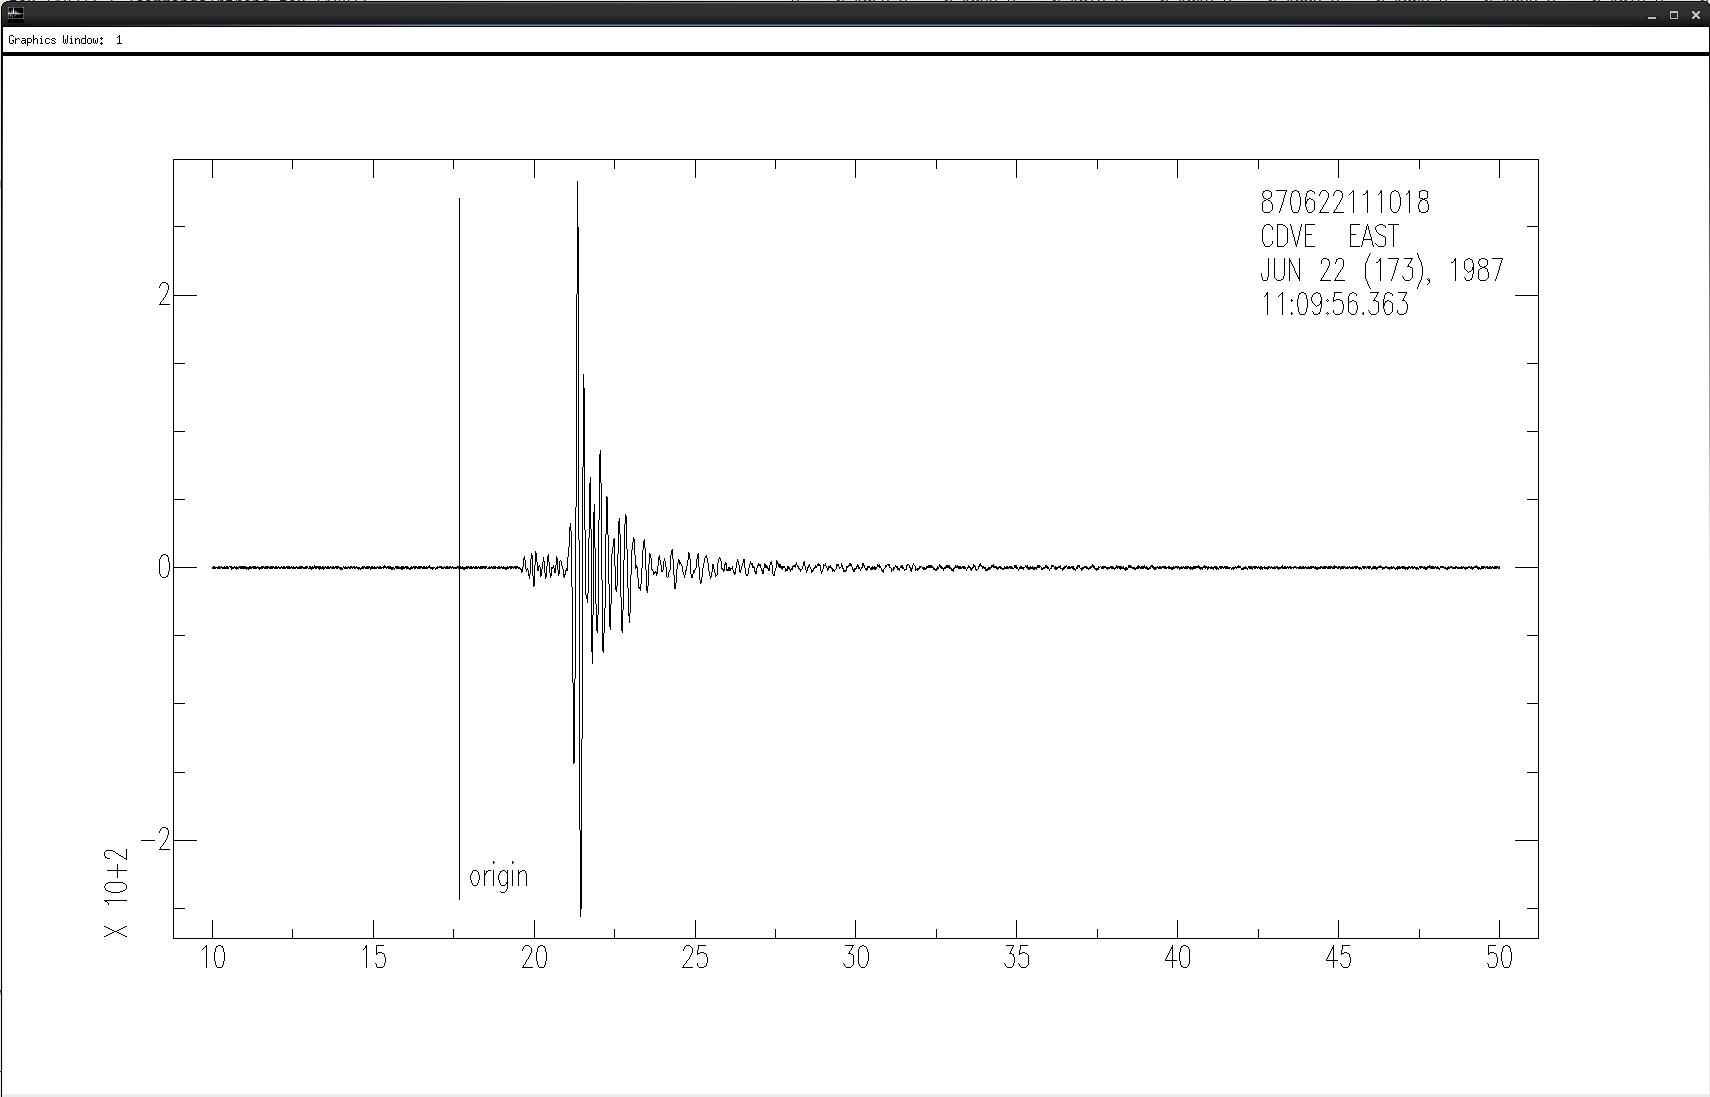
\includegraphics[width=0.9\textwidth]{plot}
\caption{绘图窗口}
\label{fig:plot}
\end{figure}

将三个波形数据读入内存,使用plot时,焦点位于绘图窗口,且绘图窗口上只显示
第一个波形,终端中出现``Waiting''字样;将焦点切换\footnote{Linux下的快捷键是Alt+Tab。}回终端,
敲击回车键,绘图窗口中显示第二个波形,终端中出现第二个``Waiting''字样,
焦点位于终端中;再次敲击回车键,窗口中显示第三个波形,焦点位于终端,
由于已经没有更多的波形需要显示,此时终端中显示SAC提示符。

如果内存中还有波形在``Waiting'',而你想要退出plot,不想要再继续查看后面的波形,
可以在终端中键入``kill''(简写为k),以直接退出plot,如下例:
\begin{SACCode}
SAC> r cdv.[nez]
SAC> p
Waitingk
SAC>
\end{SACCode}

也许你已经发现,即使plot结束或者中途退出plot,绘图窗口依然没有被关闭,而且即便
点击窗口的``关闭''按钮,窗口依然无法关闭。
\begin{SACCode}
SAC> r cdv.[nez]
SAC> begindevices xwindows      // 启动图像设备xwindows,简写为bd x
SAC> p
Waiting
Waiting
SAC> enddevices xwindows        // 关闭图像设备xwindows,简写为ed x
\end{SACCode}
严格地说,SAC绘图的流程应该是:启动图像设备(xwindows或者sgf)$\rightarrow$绘图$\rightarrow$关闭图像设备。
这样稍显繁琐,SAC将这一流程进行了简化,在每次绘图前偷偷启动了SAC默认的图像设备xwindows,
也就是上面所说的窗口,而关闭图像设备这一步需要用户自己完成,当然,在退出SAC时,SAC
也会自动关闭图像设备。

\subsection{plot1}
plot1命令会在一个窗口中显示多个波形。这些波形共用一个X轴,但拥有单独的Y轴。
\begin{SACCode}
SAC> r cdv.?
cdv.e cdv.n cdv.z
SAC> p1
\end{SACCode}
执行plot1命令后,焦点位于图形窗口,显示如图~\ref{fig:plot1}。
\begin{figure}[H]
\centering
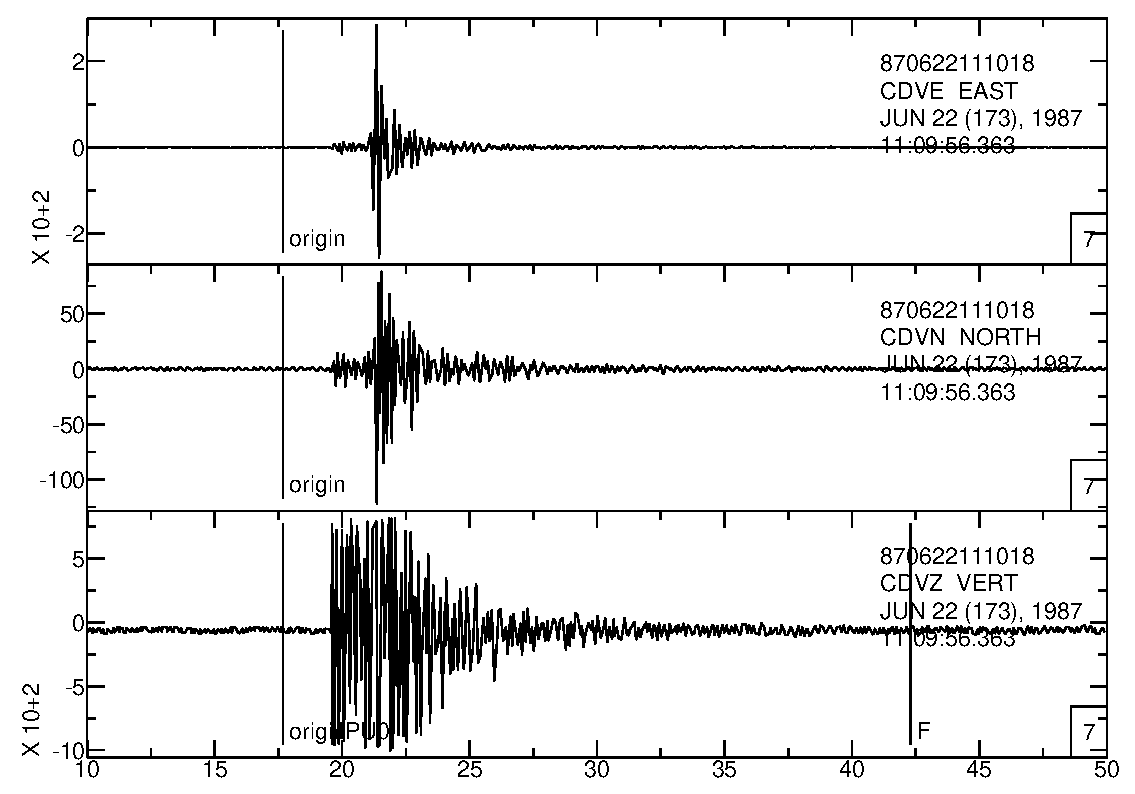
\includegraphics[width=\textwidth]{plot1}
\caption{plot1绘图效果}
\label{fig:plot1}
\end{figure}




\chapter{SAC文件格式}
\section{SAC格式简介}
一个地震波形数据包含了时间上连续的一系列数据点,数据点可以是等间隔或不等间隔采样。
SAC的数据格式要求一个文件中只包含一个地震波形数据,这样的定义更适合单个地震波形的处理。

每个SAC文件包含两个部分:一个头段区和一个数据区。

头段区位于每个文件的起始处,其大小是固定的,用于描述数据的相关信息,比如数据点数、
采样周期等等。

数据区紧跟在头段区之后,数据区又包含了一个或多个子数据区:
\begin{itemize}
\item 如果数据是时间序列,且是等间隔采样的,则只有一个子数据区,包含因变量(Y,也就是数据)的值,
    因变量(X)的信息可以直接从头段区中获得;
\item 如果数据是时间序列,但是不等间隔采样的,则有两个子数据区,分别包含因变量(Y)和自变量(X)
    的值;
\item 如果数据是谱数据而非时间序列,则有两个子数据区,分别包含振幅和相位或者实部和虚部;
\item 如果数据是三维数据(XYZ),则包含NXSIZE*NYSIZE个子数据区。
\end{itemize}

\section{两种数据形式}
SAC文件格式有两种形式:二进制型和字符型\footnote{原为alphanumeric,译为文数字。}。

字符型与二进制型是完全等价的,只是字符型是给人看的,二进制型是给机器读写的。从C
程序的角度来看,两者的区别在于,写文件时前者使用~\lstinline{fprintf}~后者使用
~\lstinline{fwrite}~。

二进制型的SAC数据,占用更小的磁盘空间,读写速度更快,因而是最常用的SAC格式形式。

字符型适合于在文件出现问题时,临时查看文件内容的时候使用。

\subsection{两种形式的互相转换}
你是否想要一个字符型的SAC文件,用编辑器打开好好看看SAC数据究竟长什么样。SAC自带
的命令可以实现两种形式的转换
\footnote{也可以使用SAC的~\lstinline{convert}~命令进行转换,不过此命令即将被淘汰。}
。
\begin{SACCode}
SAC> fg seis
SAC> w seis             // 先生成一个二进制型SAC数据,以做测试
\end{SACCode}

将二进制型转换成字符型:
\begin{SACCode}
SAC> r seis             // 读二进制型文件
SAC> w alpha seis.a     // 以字符型写入
\end{SACCode}

将字符型转换成二进制型:
\begin{SACCode}
SAC> r alpha seis.a     // 读字符型文件
SAC> w sac seis.b       // 以二进制型写入,可以省略sac,写成w seis.b
\end{SACCode}

试试用你最喜欢的文本编辑器打开字符型的~\lstinline{seis.a}~吧,其内容如下:
\begin{lstlisting}[style=Bash]
     0.01000000      -1.569280       1.520640      -12345.00      -12345.00
       9.459999       19.45000      -41.43000       10.46400      -12345.00
      -12345.00      -12345.00      -12345.00      -12345.00      -12345.00
      -12345.00      -12345.00      -12345.00      -12345.00      -12345.00
      -12345.00      -12345.00      -12345.00      -12345.00      -12345.00
      -12345.00      -12345.00      -12345.00      -12345.00      -12345.00
      -12345.00       48.00000      -120.0000      -12345.00      -12345.00
       48.00000      -125.0000      -12345.00       15.00000      -12345.00
      -12345.00      -12345.00      -12345.00      -12345.00      -12345.00
      -12345.00      -12345.00      -12345.00      -12345.00      -12345.00
       373.0627       88.14721       271.8528       3.357465      -12345.00
      -12345.00    -0.09854718       0.000000       0.000000      -12345.00
      -12345.00      -12345.00      -12345.00      -12345.00      -12345.00
      -12345.00      -12345.00      -12345.00      -12345.00      -12345.00
      1981        88        10        38        14  
         0         6         0         0      1000
    -12345    -12345    -12345    -12345    -12345
         1        50         9    -12345    -12345
    -12345    -12345        42    -12345    -12345
    -12345    -12345    -12345    -12345    -12345
    -12345    -12345    -12345    -12345    -12345
         1         1         1         1         0   
CDV      K8108838    
-12345  -12345  -12345  
-12345  -12345  -12345  
-12345  -12345  -12345  
-12345  -12345  -12345  
-12345  -12345  -12345  
-12345  -12345  -12345  
-12345  -12345  -12345  
    -0.09728001    -0.09728001    -0.09856002    -0.09856002    -0.09728001
    -0.09600000    -0.09472002    -0.09344001    -0.09344001    -0.09344001
    -0.09344001    -0.09344001    -0.09472002    -0.09472002    -0.09344001
    ......
\end{lstlisting}

第1-30行是头段区,31及以后N行是数据区。
目前你可能还看不懂头段区的这些数字或者字符代表什么。没关系,在下一节会详细介绍
SAC头段区,记得一定要一边看下一节的内容,一边对照着这个例子,好好琢磨SAC的头段。

\section{SAC头段结构}
SAC头段区长度为632个字节,由一系列头段变量构成。从这些头段变量中可以了解到波形
记录的很多信息,比如台站经纬度、发震时刻、震相到时等等。

表\ref{table:header-variables}列出了SAC头段区的全部头段变量。其中变量名为
\lstinline{internal}表示该变量为SAC内部使用的头段变量,用户不可对其进行操作。
变量名为\lstinline{unused}表示该变量暂时尚未使用,为以后可能出现的新头段变量占位。

\begin{table}[H]
\ttfamily
\small
\centering
\caption{SAC头段变量列表}
\label{table:header-variables}
\begin{tabular}{c|c|lllll}
	\toprule
    Byte	&	Type	&	\multicolumn{5}{c}{Names}\\
	\midrule
	0		&	F	&	delta	&	depmin	&	depmax	&	scale	&	odelta	\\
	20		&	F	&	b		&	e		&	o		&	a		&	internal\\
	40		&	F	&	t0		&	t1		&	t2		&	t3		&	t4		\\
	60		&	F	&	t5		&	t6		&	t7		&	t8		&	t9		\\
	80		&	F	&	f		&	resp0	&	resp1	&	resp2	&	resp3	\\
	100		&	F	&	resp4	&	resp5	&	resp6	&	resp7	&	resp8	\\
    120		&	F	&	resp9	&	stla	&	stlo	&	stel	&	stdp	\\
	140		&	F	&	evla	&	evlo	&	evel	&	evdp	&	mag		\\
	160		&	F	&	user0	&	user1	&	user2	&	user3	&	user4	\\
	180		&	F	&	user5	&	user6	&	user7	&	user8	&	user9	\\
	200		&	F	&	dist	&	az		&	baz		&	gcarc	&	internal\\
	220		&	F	&	internal&	depmen	&	cmpaz	&	cmpinc	&	xminimun\\
	240		&	F	&	xmaximum&	yminimum&	ymaximum&	unused	&	unused	\\
	260		&	F	&	unused	&	unused	&	unused	&	unused	&	unused	\\
	280		&	N	&	nzyear	&	nzjday	&	nzhour	&	nzmin	&	nzsec	\\
	300		&	N	&	nzmsec	&	nvhdr	&	norid	&	nevid	&	npts	\\
	320		&	N	&	internal&	nwfid	&	nxsize	&	nysize	&	unused	\\
	340		&	I	&	iftype	&	idep	&	iztype	&	unused	&	iinst	\\
	360		&	I	&	istreg	&	ievreg	&	ievtyp	&	iqual	&	isynth	\\
    380		&	I	&	imagtyp &	imagsrc	&	unused	&	unused	&	unused	\\
	400		&	I	&	unused	&	unused	&	unused	&	unused	&	unused	\\
	420		&	L	&	leven	&	lpspol	&	lovrok	&	lcalda	&	unused	\\
	440		&	K	&	kstnm	&	kevnm*	&			&			&			\\
	464		&	K	&	khole	&	ko		&	ka		&			&			\\
	488		&	K	&	kt0		&	kt1		&	kt2		&			&			\\
	512		&	K	&	kt3		&	kt4		&	kt5		&			&			\\
	536		&	K	&	kt6		&	kt7		&	kt8		&			&			\\
	560		&	K	&	kt9		&	kf		&	kuser0	&			&			\\
	584		&	K	&	kuser1	&	kuser2	&	kcmpnm	&			&			\\
	608		&	K	&	knetwk	&	kdatrd	&	kinst	&			&			\\
    \bottomrule
\end{tabular}
\end{table}

表\ref{table:header-variables}中,给出了头段区的全部头段变量,在源代码中,其被定义
为一个结构体,结构体中变量\lstinline{delta}开始于第零个字节,占据4个字节,
\lstinline{depmin}开始于第4个字节,也占据4个字节,其它同理。表中的第一列给出了
当前行的第一个头段变量的起始字节数。
第二列给出了头段变量的类型码,每个头段变量类型码对应的数据类型见表
\ref{sec:header-variables-type}。

表\ref{sec:header-variables-type}中,第一列为头段变量类型代码,第二类给出了其
代表的变量类型,第三列指出C源码中该变量的是用什么类型定义的,第四列给出了
写字符形式SAC文件时的输出格式。对于一个SAC文件,并非所有的头段变量都必须要包含
有意义的值,若变量未定义称其包含未定义值,第5列给出了不同类型的未定义值的形式,
比如如果一个整型头段变量的值为-12345,则认为其处于未定义态。实际使用的时候,SAC
提供了参数\lstinline{undef},其可以根据头段变量的类型自动转换成相应类型的未定义值。

SAC中定义了6种头段变量类型,分别为浮点型(F)、整型(N)、枚举型(I)、逻辑型(L)、字符型(K)和辅助型(A)。
其中辅助型不存在于SAC文件中,其直接由其它头段变量推导得到。

除了F型变量外以外,其余所有变量的变量名均以变量类型码开头,比如\lstinline{nvhdr}
是N型变量,\lstinline{leven}是L型变量。

枚举型变量,本质上是\lstinline{int}型,其只能在固定的几个值中取值;C语言中本身
是没有规定Bool类型的,SAC自定义了true和false,用于表示真和假。字符型变量长度为
8,只有\lstinline{kevnm}很特殊,其长度为16。

\begin{table}[H]
\caption{变量类型说明}
\label{table:header-variables-type}
\centering
\ttfamily
\small
\begin{tabular}{cllcll}
	\toprule
    Code    &	Type        &   C Type & sizeof &   printf	&   未定义值        \\
	\midrule
    F		&	浮点型		&   float  &  4     &	\%15.7f &   -12345.0        \\
    N		&	整型		&   int    &  4     &	\%10d   &   -12345        \\
    I		&	枚举型		&   int    &  4     &	\%10d   &   -12345	        \\
    L		&	逻辑型		&   int    &  4     &	\%10d   &   FALSE        \\
    K		&	字符型		&   char*  &  8     &	\%-8.8s & \lstinline[showspaces=true]{"-12345  "}     \\
    A		&	辅助型		&          &        &			& 	    \\
	\bottomrule
\end{tabular}
\end{table}

\section{熟悉头段变量}

\subsection{基本变量}
\begin{table}[H]
\centering
\caption{}
\label{}
\begin{tabular}{ccl}
    \toprule
	变量名	&	类型	&	描述\\
	\midrule
    nvhdr*\footnote{星号表示SAC文件中必须定义该变量}	&	N		&	SAC头段版本号,目前值为6,旧版本的SAC文件($nvhdr<6$)在读入时会自动更新。\\
	nzyear	&	N 		&	GMT年,文件参考时间	\\
    nzjday  &   N       &   GMT儒略日,一年中的第几天\footnote{比``月-日''少用一个变量。}    \\
    nzhour  &   N       &   GMT时   \\
    nzmin   &   N       &   GMT分   \\
    nzsec   &   N       &   GMT秒   \\
    nzmsec  &   N       &  GMT毫秒  \\
	nzdttm	&	N 		&	GMT日期-时间数组,不在头段中,用于子程序读取SAC文件。该数组由上面6个变量构成    \\
	kzdate	&	A		&	不在头段中,字母数字格式的GMT参考日期,由NZYEAR和NZJDAY导出\\
	kztime	&	A		&	不在头段中,字母数字格式的GMT参考时间,由NZHOUR, NZMIN, NZSEC和NZMSEC导出\\
	iftype*	&	I		&	文件类型:\\
						&& \quad- ITIME 时间序列文件	\\
						&& \quad- IRLIM 频谱文件实部-虚部格式 \\
 						&& \quad- IAMPH 频谱文件振幅-相位格式	\\
						&& \quad- IXY 一般的x-y数据 	\\
						&& \quad- IXYZ 一般的XYZ(3-D)文件\\	
	idep	&	I		&	因变量类型:\\
						&& \quad- IUNKN (未知)	\\
						&& \quad- IDISP (位移:nm)	\\
						&& \quad- IVEL (速度:nm/sec)	\\
						&& \quad- IVOLTS (速度:volts)	\\
						&& \quad- IACC (加速度:nm/sec/sec)	\\
	iztype	&	I 		&	等效参考时间	\\
						&& \quad- IUNKN (未知)	\\
						&& \quad- IB (文件开始时间)	\\
						&& \quad- IDAY (基准GMT的午夜)	\\
						&& \quad- IO (事件发生时间)	\\
						&& \quad- IA (初动到时)	\\
						&& \quad- ITn (用户自定义的读取时间Tn, n=0,9)	\\
    \bottomrule
\end{tabular}
\end{table}

\subsection{数据相关变量}
\begin{table}[H]
\centering
\caption{}
\label{}
\begin{tabular}{ccc}
    \toprule
	变量名	&	类型	&	描述\\
	\midrule
    npts*	&   N		&	数据点数。\\
	delta*	&	F		&	等间隔数据的采样间隔(标称值)。\\
	DEPMIN	&	F 		&	因变量最小值。	\\
	DEPMAX	&	F		&	因变量最大值	\\
	DEPMEN	&	F		&	因变量平均值	\\
	SCALE	&	F		&	因变量比例因子\footnote{真实物理场被乘以比例因子得到现有数据}	\\
	ODELTA*	&	F		&	采样间隔的观测值,若观测值与标称值不同则有值\\
	B*		&	F		&	自变量起始值(相对参考时间的秒数)\\
	E*		&	F		&	自变量结束值(相对参考时间的秒数)\\
    XMINIMUM&   F       &   X的最小值(限于谱文件)   \\                                                                                                    
    XMAXIMUM&   F       &   X的最大值(限于谱文件)   \\                           
    YMINIMUM&   F       &   Y的最小值(限于谱文件)   \\                           
    YMAXIMUM&   F       &   Y的最大值(限于谱文件)   \\  
    NXSIZE  &   N       &   频谱长度(限于谱文件)    \\                           
    NYSIZE  &   N       &   频谱宽度(限于谱文件)    \\
    IQUAL   &   I       &   数据质量[未使用]:   \\                                                                                                        
                        && - IGOOD (Good data)  \\                               
                        && - IGLCH (Glitches)   \\                               
                        && - IDROP (Dropouts)   \\                               
                        && - ILOWSN (Low signal to noise ratio) \\               
                        && - IOTHER (Other)\\                                    
    ISYNTH  &   I       &   合成数据标识[未使用]:\\                              
                        && - IRLDTA (Real data) \\                               
                        && - ????? (Flags for various synthetic seismogram codes) \\
     LEVEN*  &   L       &   若数据为等间隔则为TRUE。\\
    \bottomrule
\end{tabular}
\end{table}

\subsection{事件相关变量}
\begin{table}[H]
\centering
\caption{}
\label{}
\begin{tabular}{ccc}
    \toprule
	变量名	&	类型	&	描述\\
	\midrule
    KEVNM   &   K       &   事件名  \\
    IEVREG  &   I       &   事件地理区域[未使用]    \\
    IEVTYP  &   I       &   事件类型    \\
    EVLA    &   F       &   事件纬度(度,北为正) \\                                                                                                        
    EVLO    &   F       &   事件经度(度,东为正) \\                                  
    EVEL    &   F       &   事件高程(m). [未使用]   \\                              
    EVDP    &   F       &   事件相对地表深度(m). [未使用]   \\                   
    MAG     &   F       &   事件震级    \\                                       
    IMAGTYP &   I       &   震级类型:\\                       
    IMAGSRC &   I       &   震级来源信息:   \\
    NEVID   &   N       &   事件ID (CSS 3.0)    \\
    NORID   &   N       &   起始时间ID (CSS 3.0)    \\ 
    NWFID   &   N       &   波形ID (CSS 3.0)    \\ 
    KHOLE   &   K       &   核爆事件:孔眼标识;其他:位置标识  \\
    GCARC   &   F       &   台站到事件的大园弧长,即另一种震中距(度).\\ 
    DIST    &   F       &   事件台站距离,即震中距(km)\\                         
    AZ      &   F       &   事件到台站的方位角(度).\\                                                                                                     
    BAZ     &   F       &   台站到事件的方位角(度). \\                           
    O       &   F       &   事件发生时间(相对参考时间的秒数)    \\                                                                                        
    KO      &   A       &   事件发生时间标志    \\  
    \bottomrule
\end{tabular}
\end{table}

\subsection{台站相关变量}
\begin{table}[H]
\centering
\caption{}
\label{}
\begin{tabular}{ccc}
    \toprule
	变量名	&	类型	&	描述\\
    \midrule
    KNETWK  &   K       &   地震台网名  \\
    KSTNM   &   K       &   台站名      \\      
    ISTREG  &   I       &   台站地理区域[未使用]    \\  
    STLA    &   F       &   台站纬度(度,北为正)    \\                           
    STLO    &   F       &   台站经度(度,东为正).   \\                           
    STEL    &   F       &   台站高程(m). [未使用]\\                              
    STDP    &   F       &   台站相对地表深度(m). [未使用]\\                      
    CMPAZ   &   F       &   分量方位角(从北开始顺时针度数).\\                    
    CMPINC  &   F       &   分量倾角(从垂直开始的度数)  \\    
    KCMPNM  &   K       &   分量名称,SEED格式使用那个三字符名称,第三个代表分量的方位(如BHE),
                            对于水平分量,目前的趋势是使用1和2代替N和E  \\ 
    KSTCMP  &   A       &   台站分量,由KSTNM, CMPAZ和CMPINC导出\\
    LPSPOL  &   L       &   如果台站分量为正极性则为真(左手规则)  \\
    \bottomrule
\end{tabular}
\end{table}

\subsection{震相相关变量}
\begin{table}[H]
\centering
\caption{}
\label{}
\begin{tabular}{ccc}
    \toprule
	变量名	&	类型	&	描述\\
    \midrule
    A       &   F       &   初动到时(相对参考时间的秒数)\\                       
    KA      &   K       &   初动到时标志    \\                                                                                                            
    F       &   F       &   事件结束时间(相对参考时间的描述,注意与文件结束时间的区别)\\
    KF      &   A       &   事件结束标志    \\                                   
    Tn      &   F       &   用户定义的时间,在拾取震相时使用,n = 0-9(相对参考时间的秒数)\\
    KTn     &   K       &   用户定义的时间标志, n = 0-9.    \\ 
    \bottomrule
\end{tabular}
\end{table}

\subsection{仪器相关变量}
\begin{table}[H]
\centering
\caption{}
\label{}
\begin{tabular}{ccc}
    \toprule
	变量名	&	类型	&	描述\\
    \midrule
    KINST   &   K       &   记录仪器通用名称    \\                               
    IINST   &   I       &   记录仪器类型[未使用]\\                               
    RESPn   &   F       &   仪器响应参数,n=0,9. [未使用]\\
    \bottomrule
\end{tabular}
\end{table}

\subsection{其它变量}
\begin{table}[H]
\centering
\caption{}
\label{}
\begin{tabular}{ccc}
    \toprule
	变量名	&	类型	&	描述\\
    \midrule
    USERn   &   F       &   用户定义变量存储区, n = 0,9.\\
    KUSERn  &   K       &   用户定义变量存储区,  n = 0,9.\\     
    LOVROK  &   L       &   如果文件可覆盖则为真,类似于写权限  \\  
    LCALDA  &   L       &   如果DIST, AZ, BAZ 和 GCARC可以由台站和事件的坐标计算出来则为真\\
    KDATRD  &   K       &   数据被读入计算机的日期\\ 
    \bottomrule
\end{tabular}
\end{table}

\section{SAC中的时间概念}
\label{sec:sac-time}

\subsection{基本思路}
SAC的头段区有很多与时间相关的头段变量,包括nzyear、nzjday、nzhour、nzmin、nzsec、
nzmsec、b、e、o、a、f、tn(n=0-9),正确使用它们的前提是理解SAC中的时间概念。
这一节将试着说清楚这个问题。

首先,SAC处理的是地震波形数据,SAC格式里保存的是时间序列数据。先不管其它的一些台站
经纬度、事件经纬度信息,就数据而言,至少需要一系列数据值以及每个数据值所对应的时刻。

在本节接下来的内容中,将严格区分两个高中物理学过的概念:时刻和时间。简单地说,
在时间轴上,时刻是一个点,时间是一个线段。

一个简单的例子如下:
\begin{lstlisting}[style=Bash]
2014-02-26T20:45:00.000     0.10
2014-02-26T20:45:01.000     0.25
2014-02-26T20:45:02.000     0.33
2014-02-26T20:45:03.000     0.21
2014-02-26T20:45:04.000     0.35
2014-02-26T20:45:05.000     0.55
2014-02-26T20:45:06.000     0.78
2014-02-26T20:45:07.000     0.66
2014-02-26T20:45:08.000     0.42
2014-02-26T20:45:09.000     0.34
2014-02-26T20:45:10.000     0.25
\end{lstlisting}
其中第二列是数据点,每个数据点所对应的时刻放在第一列,格式为``yyyy-mm-ddThh:mm:ss.xxx''。
数据点是以1s的等间隔进行采样的。

若把这堆时刻以及数据点直接写入文件中,将占据大量的磁盘空间,读写也很不方便。
考虑将某一个时刻定义为参考时刻,并把其它所有的时刻都用相对于该参考时刻的时间来表示。
这样可以简化不少。

比如取``\lstinline{2014-02-26T20:45:00.000}''为参考时刻,即
\begin{lstlisting}[style=Bash]
nzyear = 2014
nzjday = 57
nzhour = 20
nzmin  = 45
nzsec  = 00
nzmsec = 000
\end{lstlisting}
则上面的数据可以简化为
\begin{lstlisting}[style=Bash]
00.000     0.10
01.000     0.25
02.000     0.33
03.000     0.21
04.000     0.35
05.000     0.55
06.000     0.78
07.000     0.66
08.000     0.42
09.000     0.34
10.000     0.25
\end{lstlisting}
其中第二列是数据点,第一列是每个数据点对应的时刻相对于参考时刻的相对时间,下面
简称其为相对时间。

显然参考时刻的选取是任意的,若取``\lstinline{2014-02-26T20:45:05.000}''为参考时刻,
则上面的数据简化为
\begin{lstlisting}[style=Bash]
-05.000     0.10
-04.000     0.25
-03.000     0.33
-02.000     0.21
-01.000     0.35
 00.000     0.55
 01.000     0.78
 02.000     0.66
 03.000     0.42
 04.000     0.34
 05.000     0.25
\end{lstlisting}

一般来说,会选取一个比较特殊的时刻作为参考时刻,比如第一个数据点对应的时刻,或者
地震波形数据中的发震时刻。

下面还是回到以``\lstinline{2014-02-26T20:45:00.000}''为参考时刻简化得到的结果。
因为数据是等间距的,相对时间这一列完全可以进一步简化,比如用``起始相对时间+采样间隔
+数据点数''或者``起始相对时间+采样间隔+结束相对时间''就完全可以表征第一列的相对
时间。如果只能从二者之中选一个的话,我会选择第一种,毕竟``数据点数''太有用了。

SAC选择了另外一种简化模式,``起始相对时间+采样间隔+数据点数+结束相对时间'',即
头段变量中的``\lstinline{ b + delta + npts + e }'',这其实是存在数据冗余的,这就
造就了头段变量\lstinline{e}的一些特殊性,后面会提到。

按照SAC的模式再对相对时间进行简化之后,整个数据可以表示为
\begin{lstlisting}[style=Bash]
nzyear = 2014 
nzjday = 57
nzhour = 20
nzmin  = 45
nzsec  = 00
nzmsec = 000
b      = 0.0
e      = 10.0
delta  = 1.0
npts   = 11

0.10
0.25
0.33
0.21
0.35
0.55
0.78
0.66
0.42
0.34
0.25
\end{lstlisting}

似乎到这里就结束了。

地震学里的一个重要问题是拾取震相到时(时刻),所以还需要几个额外的头段变量来保存
这些震相到时(时刻),不过显然我们不会真的把时刻保存到这些头段变量中,不然上面的
一大堆就真是废话了。SAC将震相到时(时刻)相对于参考时刻的时间差(即相对时间)保存
到头段变量o、a、f、tn中。

综上,SAC中跟时间有关的概念有三个:
\begin{description}
    \item [参考时刻] 保存到头段变量nzyear、nzjday、nzhour、nzmin、nzsec、nzmsec中;
    \item [相对时间] 即某个时刻相对于参考时刻的时间差(单位为秒),保存到头段变量b、e
    o、a、f、tn;
    \item [绝对时刻] =参考时刻+相对时间;
\end{description}

\subsection{在测试中学会领悟}
下面以一个具体的数据为例,通过修改各种与时间相关的头段来试着去进一步理解SAC的时间概念。

\subsubsection{生成样例数据}
\begin{SACCode}
SAC> fg seis
SAC> lh iztype

  FILE: SEISMOGRAM - 1
   ------------

    iztype = BEGIN TIME
SAC> ch iztype IUNKN
SAC> w seis
\end{SACCode}
lh是命令\nameref{cmd:listhdr}的简写,用于列出头段变量的值。ch是\nameref{cmd:chnhdr}
的简写,用于修改头段变量的值。

这里额外多做了一个操作修改iztype的操作,这是由于这个数据稍稍有一点bug。

iztype指定了参考的类型,其显示为BEGIN TIME,实际上其枚举值是IB,也就是说这个数据
选取文件第一个数据点的时刻作为参考时刻,那么b的值应该为0。而实际上这个数据的b值
并不为0,这其实就这个数据的一点小bug。这也从另一个侧面说明
SAC只有在修改与时间相关的头段变量时才可能会检查到这个错误/警告,所以这里
先将其修正为IUNKN。

\subsubsection{修改文件起始时间b}
\begin{SACCode}
SAC> r seis
SAC> lh kzdate kztime b delta npts e o a f
  
  FILE: seis - 1
 --------------

     kzdate = MAR 29 (088), 1981
     kztime = 10:38:14.000
          b = 9.459999e+00
      delta = 1.000000e-02
       npts = 1000
          e = 1.945000e+01
          o = -4.143000e+01
          a = 1.046400e+01
SAC> ch b 10
SAC> lh
  
  FILE: seis - 1
   ----------

     kzdate = MAR 29 (088), 1981
     kztime = 10:38:14.000
          b = 1.000000e+01
      delta = 1.000000e-02
       npts = 1000
          e = 1.999000e+01
          o = -4.143000e+01
          a = 1.046400e+01
\end{SACCode}

修改b前后的变化仅在于b和e值的变化,而参考时刻以及其它相对时间并没有发生变化。

这意味着整段SAC数据中的任意一个数据点所对应的时刻\footnote{好长的修饰语}都向后
延迟了0.54秒!这样做很危险,因为b和e的绝对时刻被修改了,而其它头段如o、a、f、tn的
绝对时刻却没有变。

使用的时候必须非常小心:
\begin{itemize}
\item 如果o、a、f、tn都没有定义,那么修改b值可以用于校正仪器的时间零飘\footnote{零飘,
    即仪器中的时刻与标准时刻不同。}以及时区差异\footnote{时区差异可以理解成另一种零飘。}。
\item 如果o、a、f、tn已经被定义,则修改b值会引起这些震相相关的头段变量出现错误!
    \footnote{如果只定义了o值,或者a、f、tn为理论震相到时而非计算机拾取或人工拾取的
    到时,修改b也是没有问题的。有些乱,不多说了。}
\end{itemize}

\subsubsection{修改文件结束时间e}
\begin{SACCode}
SAC> r ./seis 
SAC> lh kzdate kztime b delta npts e o a f 
  
  FILE: ./seis - 1
 ------------

     kzdate = MAR 29 (088), 1981
     kztime = 10:38:14.000
          b = 9.459999e+00
      delta = 1.000000e-02
       npts = 1000
          e = 1.945000e+01
          o = -4.143000e+01
          a = 1.046400e+01
SAC> ch e 0
SAC> lh
  
  FILE: ./seis - 1
 ------------

     kzdate = MAR 29 (088), 1981
     kztime = 10:38:14.000
          b = 9.459999e+00
      delta = 1.000000e-02
       npts = 1000
          e = 1.945000e+01
          o = -4.143000e+01
          a = 1.046400e+01
\end{SACCode}

可以看到,修改前后所有变量均没有发生变化,即e的值是不可以随意改变的,根据上面的
结果可知,e的值是通过b、delta、npts的值动态计算的。这也与上一节说到的头段变量
冗余问题相符合。不要试图修改delta、npts,这不科学!

\subsubsection{修改o、a、f、tn}
这几个头段变量完全是由用户自定义的,因而任何的定义、修改、取消定义都不会对数据
的正确性产生影响,因而这里不再测试。

\subsubsection{修改参考时间}
\begin{SACCode}
SAC> r ./seis 
SAC> lh kzdate kztime b delta npts e o a f
  
  FILE: ./seis - 1
 ------------

     kzdate = MAR 29 (088), 1981
     kztime = 10:38:14.000
          b = 9.459999e+00
      delta = 1.000000e-02
       npts = 1000
          e = 1.945000e+01
          o = -4.143000e+01
          a = 1.046400e+01
SAC> ch nzsec 15
SAC> lh
  
  FILE: ./seis - 1
 ------------

     kzdate = MAR 29 (088), 1981
     kztime = 10:38:15.000
          b = 9.459999e+00
      delta = 1.000000e-02
       npts = 1000
          e = 1.945000e+01
          o = -4.143000e+01
          a = 1.046400e+01

\end{SACCode}

试图修改参考时刻,整个SAC头段,除了参考时刻外其它时间变量都没有发生变化。根据
``绝对时刻=参考时刻+相对时刻''可知,这导致所有SAC数据点的绝对时刻发生了平移,
这一点理论上可以用于校正零飘或者时区,但是由于SAC不支持智能判断时间(比如不知道
1时80分实际上是2时20分),所以修改时区时需要获取参考时刻6个头段变量,加上时区的
校正值,再写入到参考时刻6个变量中,相对较为繁琐。

\subsubsection{修改发震时刻}
数据处理中一个常见的需求是修改发震时刻,这可以通过修改头段变量o来实现,但是经常
需要将参考时刻设置为发震时刻。
上面的测试表明,直接修改参考时刻是很危险的,所以SAC的ch命令提供了allt选项,来实现
这一功能,在\nameref{sec:origin-time}一节中会具体解释。

\subsection{总结}
将SAC中的时间变量分为三类:
\begin{enumerate}
\item 参考时刻:即nzyear、nzjday、nzhour、nzmin、nzsec、nzmsec;
\item 相对时间:即o、a、f、tn;
\item 特殊的相对时间:即b\footnote{由于e不可独立修改,所以不再考虑};
\end{enumerate}

第二类时间变量可以随意修改,即震相拾取。

第一、三类时间变量的修改会导致数据绝对时刻发生改变,可用于校正时间零飘或时区
不一致问题。

而为了修改发震时刻(此时应保证数据的绝对时刻不发生改变),则需要使用ch提供的allt
选项来实现。




\backmatter

\end{document}
